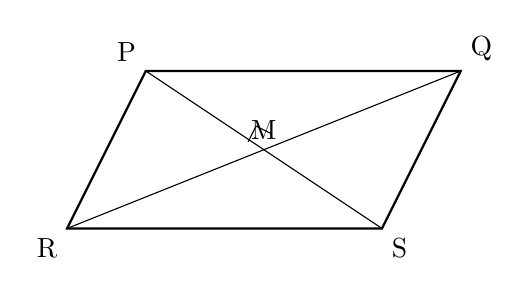
\begin{tikzpicture}
    % Parallelogram
    \draw[thick] (0,0) coordinate (R) -- (4,0) coordinate (S) -- (5,2) coordinate (Q) -- (1,2) coordinate (P) -- cycle;
    
    % Diagonals
    \draw (P) -- (S);
    \draw (R) -- (Q);
    
    % Intersection M
    \coordinate (M) at (2.5,1);
    \node[above] at (M) {M};
    
    % Labels
    \node[above left] at (P) {P};
    \node[above right] at (Q) {Q};
    \node[below right] at (S) {S};
    \node[below left] at (R) {R};
    
    % Measurements
    %\node[below] at (3,2.7) {PQ = 5 cm};
    %\node[right] at (3.5,0.5) {MQ = 4 cm};
    
    % Right angle at M
    \draw (2.3,1.1) -- (2.4,1.3) -- (2.6,1.2);
\end{tikzpicture}